%===================================== CHAP 5 =================================

\chapter{Experimental testing}
This chapter contain the result from the test that were performed. The goal with these test was to evaulate the ublox receiver againgst the pixi receiver, and to get a impresion on the accuracy to the rtklib solution with ublox. The comparison test was performed with the pixi and ublox connected to the same antenna at both the rover and the base station. Then the deviation in the position estimate can only come from the receivers. The accuracy test of the ublox was tested by performing the same manoeuvre several times.

All position and velocity data is given in the \gls{ned} frame. 
Can mension the gnss radar used to find good gps windows.
\section{Physical testing}
The physical experiment were done in two parts. During the first part the x8 was carried around on a open field. The goal with this experiment was to log data from rtklib and piksi, and then compare how they deviated from each other. The second part of the physical experiment was flying (SKRIV NÅR FLYVING ER GJENNNOMFØRT)

\subsection{GPS test}
In this part two sessions of navigation data will be presented. Both sessions were performed on the same day, which was cloudless and at a time with low \gls{dop}. The raw data from the Ublox receiver was post processed with rtklib, and is should be more accurate than it's real time counter part. Therefore a error was defined as:
\begin{equation}
e(t) = p_r(t) - p_p(t)
\end{equation}
where $p_r(t)$ and $p_p(t)$ is defined as the position solution from the real time system and the position solution from the post processed solution respectfully. It should be noted that in order to compare the different time-series the position data was synchronized with each other. From the error the cumulative mean error and cumulative standard deviation for the error was calculated using the matlab function "mean" and "std".

Figure \ref{figure:xywalk1} shows a North East plot of how the walk was. The plot contain only the fixed solution from both the piksi and rtklib. 
\begin{figure}[H]
	\centering
		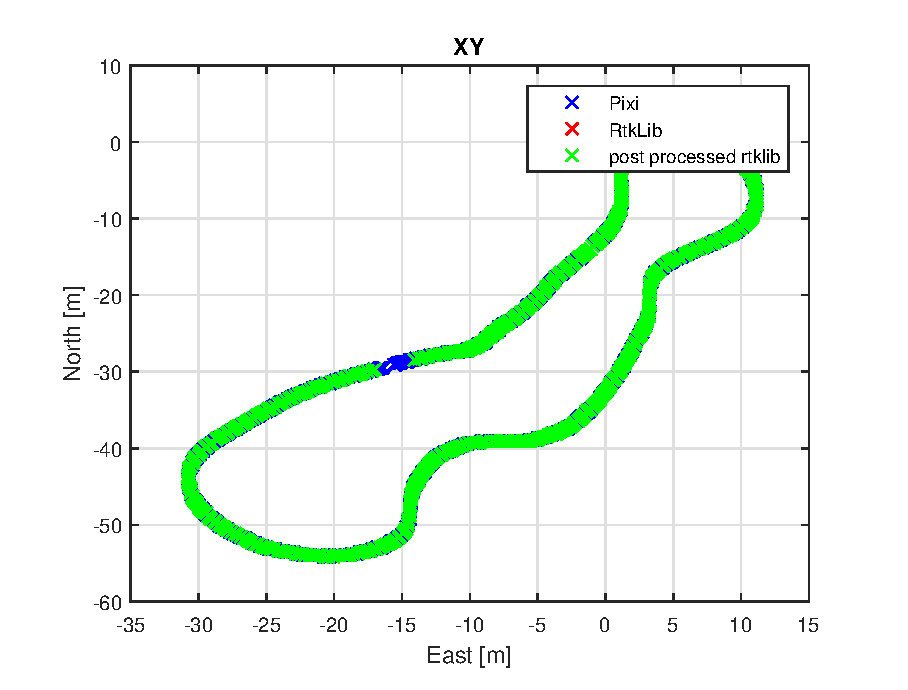
\includegraphics[width=0.7\textwidth]{figs/plots/xy.eps}
		\caption{A xy plot of the piksi,rtklib real time solution and the rtklib post processed solution}
		\label{figure:xywalk1}
\end{figure}
Figure \ref{figure:DownAndAmbwalk1} shows the down position, as well as how the integer ambiguity solution was during the experiment. As seen in the figure both the Piksi and Rtklib manage to keep there fixed solution. The position solution from both the Piksi and Rtklib agrees with the post processed solution. 
\begin{figure}[H]
	\centering
		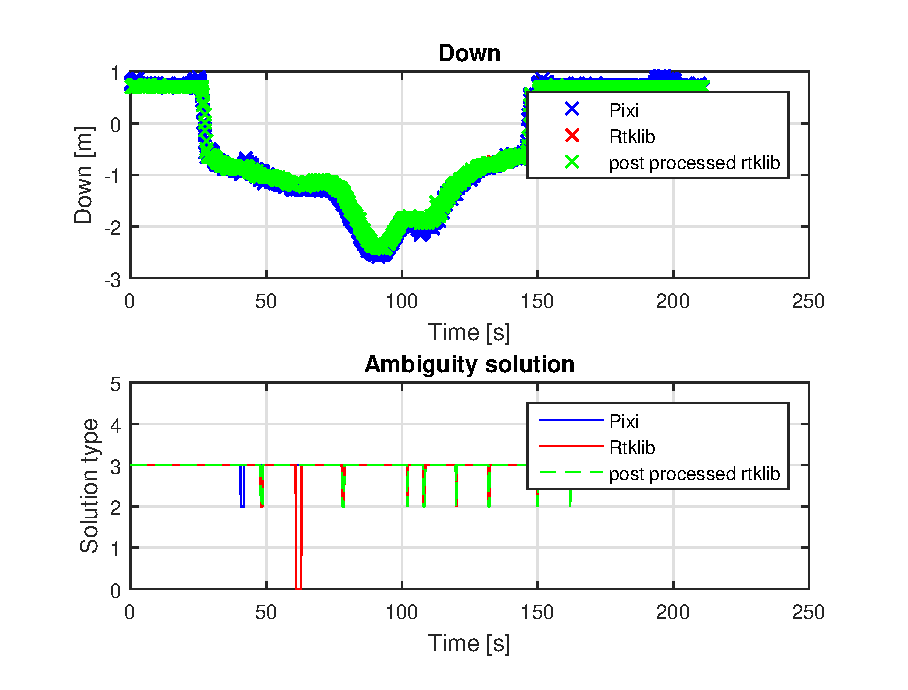
\includegraphics[width=0.7\textwidth]{figs/plots/down.eps}
		\caption{The communication structure of rtklib}
		\label{figure:DownAndAmbwalk1}
\end{figure}

As seen in figure \ref{figure:xywalk1} the difference between the different solution appear to be small, which is comfirmed in the error plot shown in figure \ref{figure:errorRTKwalk1} and \ref{figure:errorPiksiwalk1}
\begin{figure}[H]
	\centering
		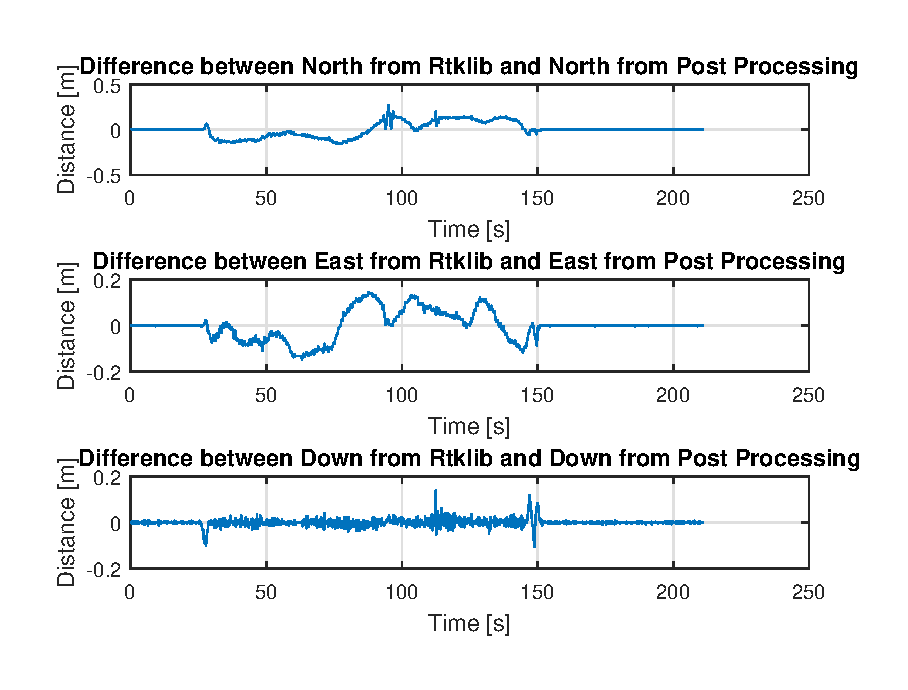
\includegraphics[width=0.7\textwidth]{figs/plots/ertkpost.eps}
		\caption{The difference between rtklib real time and post processed solution}
		\label{figure:errorRTKwalk1}
\end{figure}
\begin{figure}[H]
	\centering
		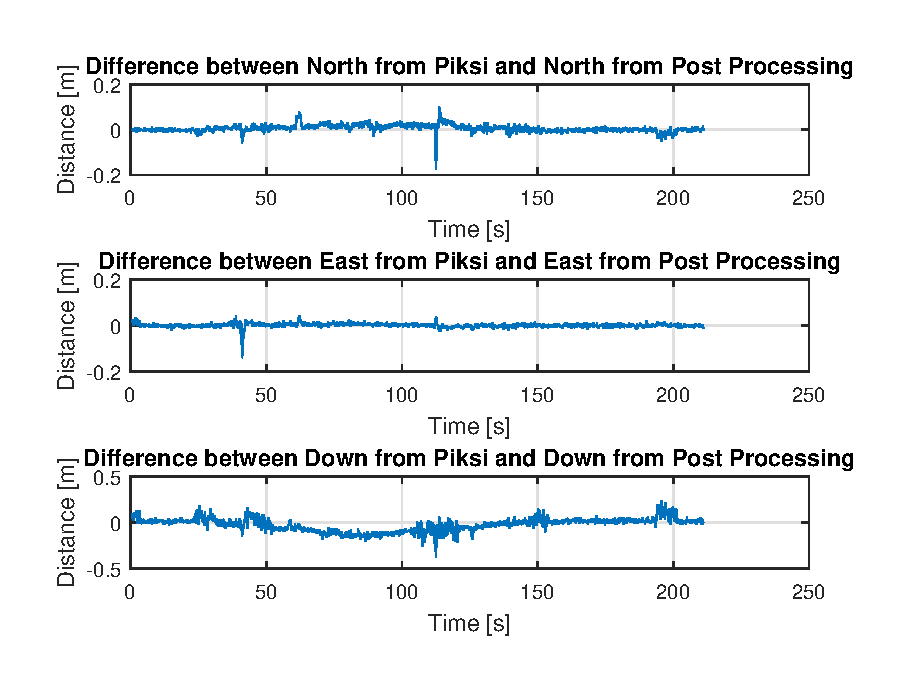
\includegraphics[width=0.7\textwidth]{figs/plots/epiksiport.eps}
		\caption{The communication structure of rtklib}
		\label{figure:errorPiksiwalk1}
\end{figure}
\begin{figure}[H]
	\centering
		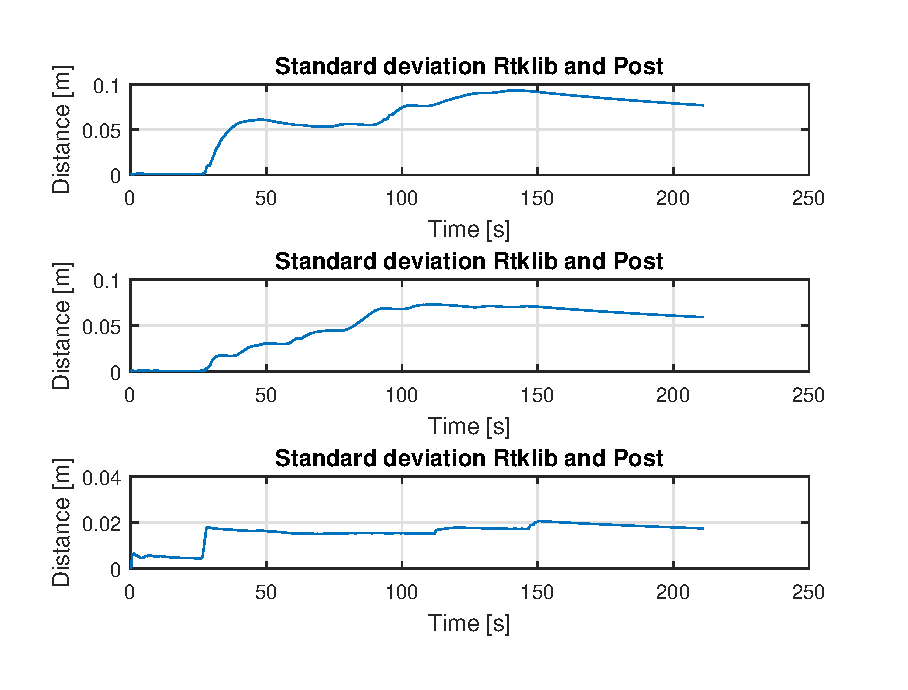
\includegraphics[width=0.7\textwidth]{figs/plots/stdrtkpost.eps}
		\caption{Standard deviation of the difference between rtklib real time and post processed solution}
		\label{figure:RTKLIB_STRUCTURE}
\end{figure}
\begin{figure}[H]
	\centering
		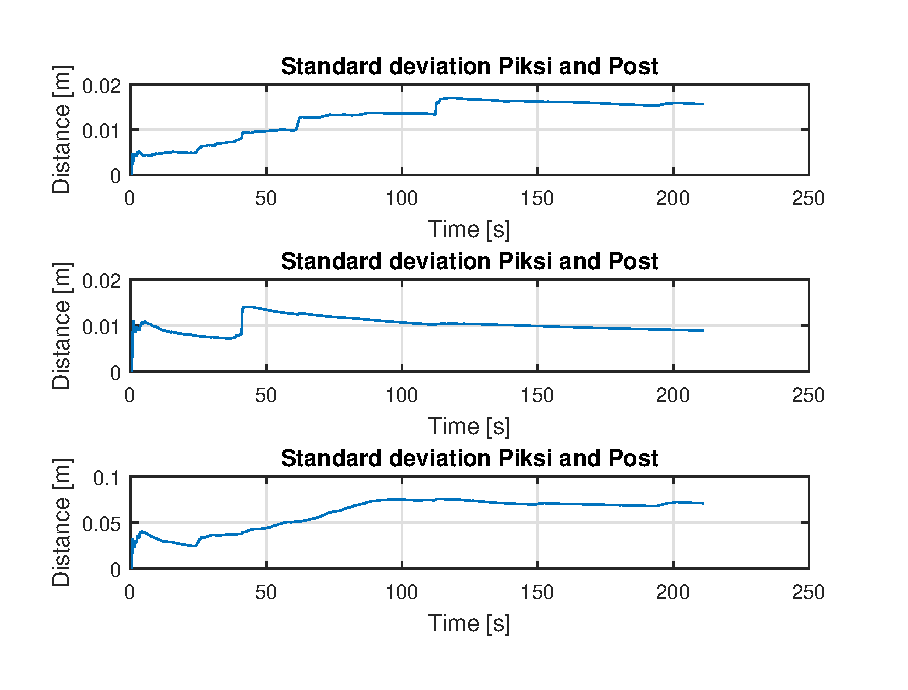
\includegraphics[width=0.7\textwidth]{figs/plots/stdpiksipost.eps}
		\caption{Standard deviation of the difference between piksi real time and rtklib post processed solution}
		\label{figure:RTKLIB_STRUCTURE}
\end{figure}

\begin{figure}[H]
	\centering
		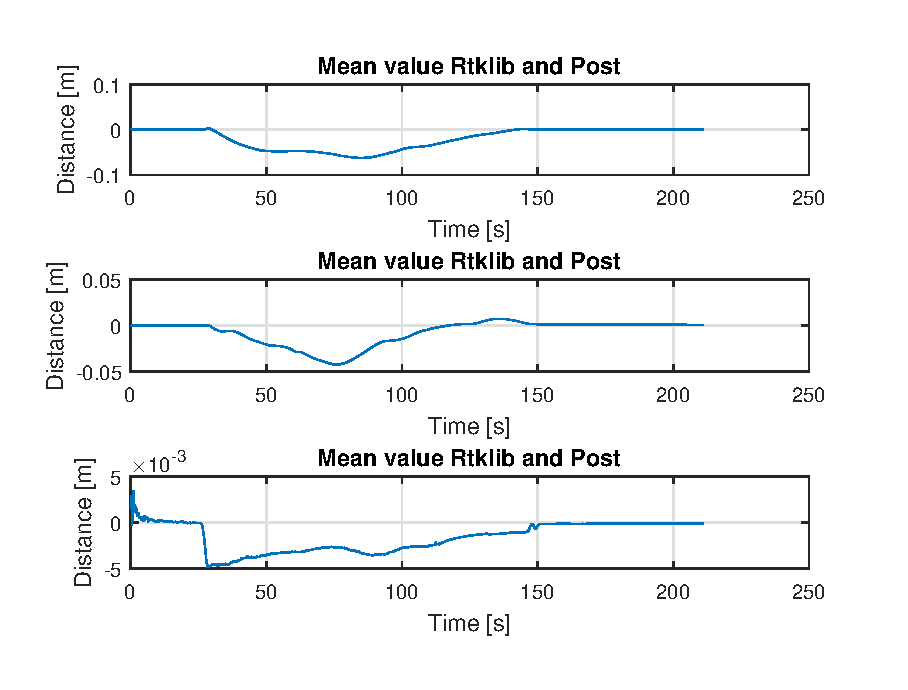
\includegraphics[width=0.7\textwidth]{figs/plots/meanrtkpost.eps}
		\caption{The mean difference between the rtklib real time and post processed solution}
		\label{figure:RTKLIB_STRUCTURE}
\end{figure}
\begin{figure}[H]
	\centering
		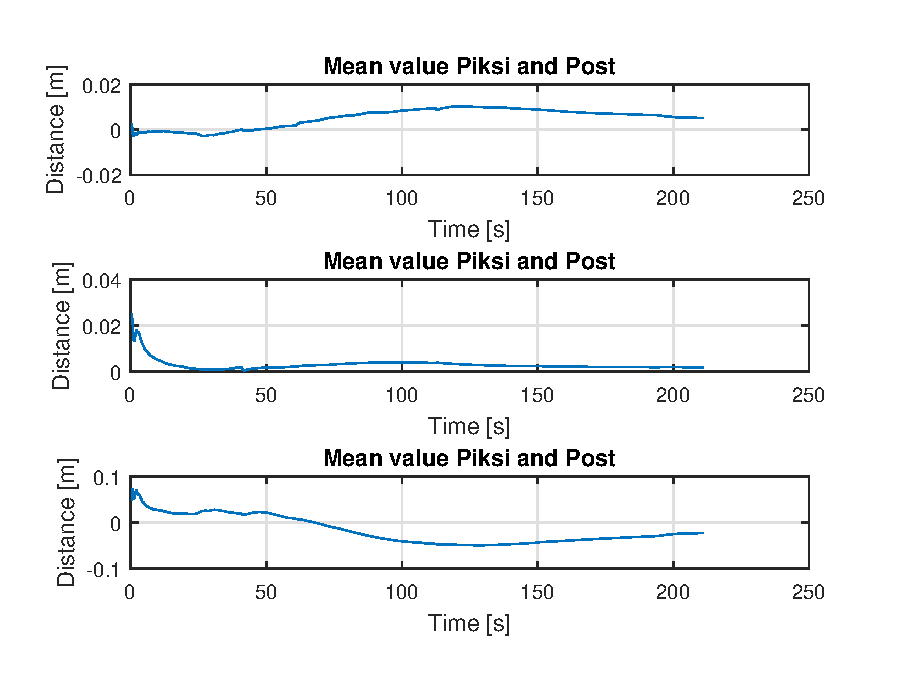
\includegraphics[width=0.7\textwidth]{figs/plots/meanpiksipost.eps}
		\caption{The mean difference between the piksi real time and the rtklib post processed solution}
		\label{figure:RTKLIB_STRUCTURE}
\end{figure}
The velocity data is shown in figure \ref{figure:VelocityWalk1}. It appears that rtklib has a delayed solution, that might be because of problem with the \gls{tow} that was identified in rtklib.
\begin{figure}[H]
	\centering
		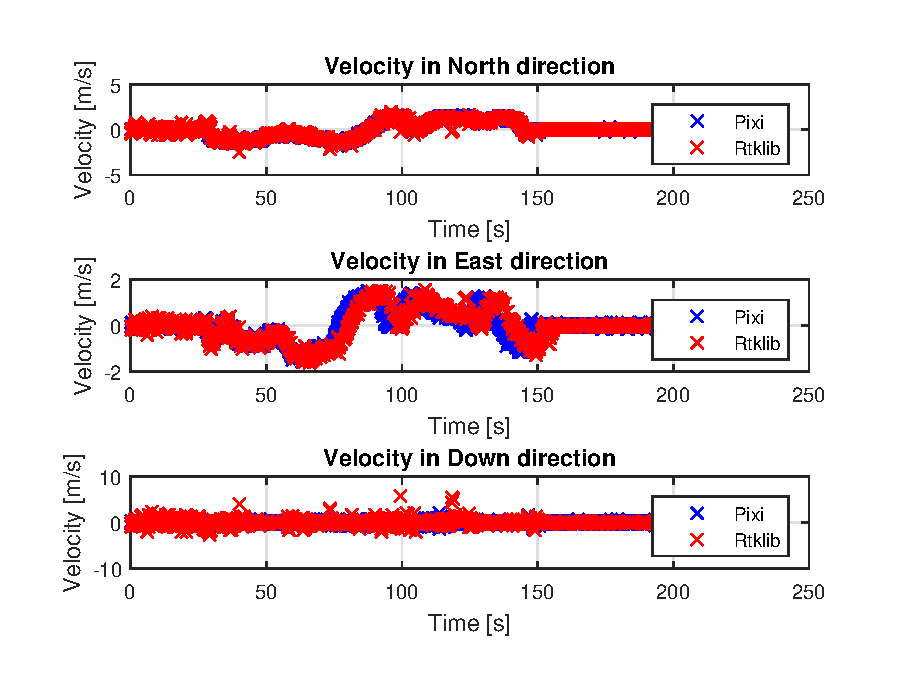
\includegraphics[width=0.7\textwidth]{figs/plots/velocity.eps}
		\caption{Velocity data from the piksi and rtklib real time solution}
		\label{figure:VelocityWalk1}
\end{figure}
The problem with the \gls{tow} is shown more clearly in figure \ref{figure:timeRTKwalk1}. The figure display the time difference between each output. The first part is an altered version of the \gls{tow} from rtklib, while the other is the timestamp of the same output given by Dune. The output from rtklib gave only seconds, and not a millisecond value. To correct for this error the \gls{tow} value from rtklib altered to fill the gap between each second. The alteration was done by counting the number of elements with the same \gls{tow} value, and then equally spread them from between the \gls{tow} value to the next \gls{tow} value.

The timestamp given by Dune indicate the delay a output message from rtklib might experience before it's available for consumption. Both the timestamp and \gls{tow} value indicate that rtklib has a mean output of 5 Hz. 
\begin{figure}[H]
	\centering
		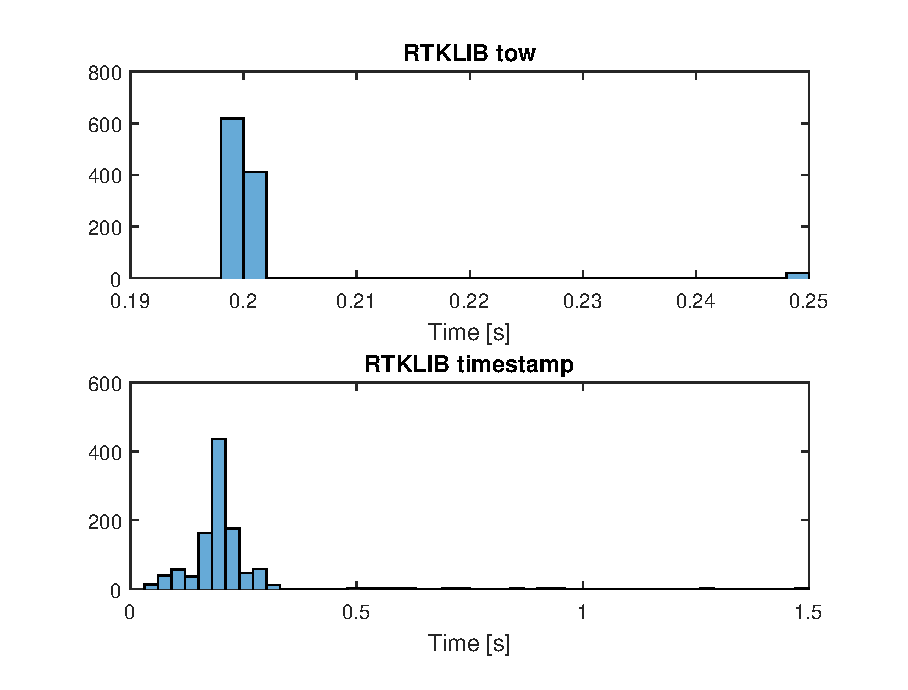
\includegraphics[width=0.7\textwidth]{figs/plots/rtktime.eps}
		\caption{The time between time samples from rtklib}
		\label{figure:timeRTKwalk1}
\end{figure}
Figure \ref{figure:timePiksiWalk1} shows the time difference between each output sample. The first plot shows the difference between each \gls{tow} value from Piksi, and the other the difference between each time stamp given by Dune. Both plots indicate that Piksi is able to have a output frequency at 10 Hz.
\begin{figure}[H]
	\centering
		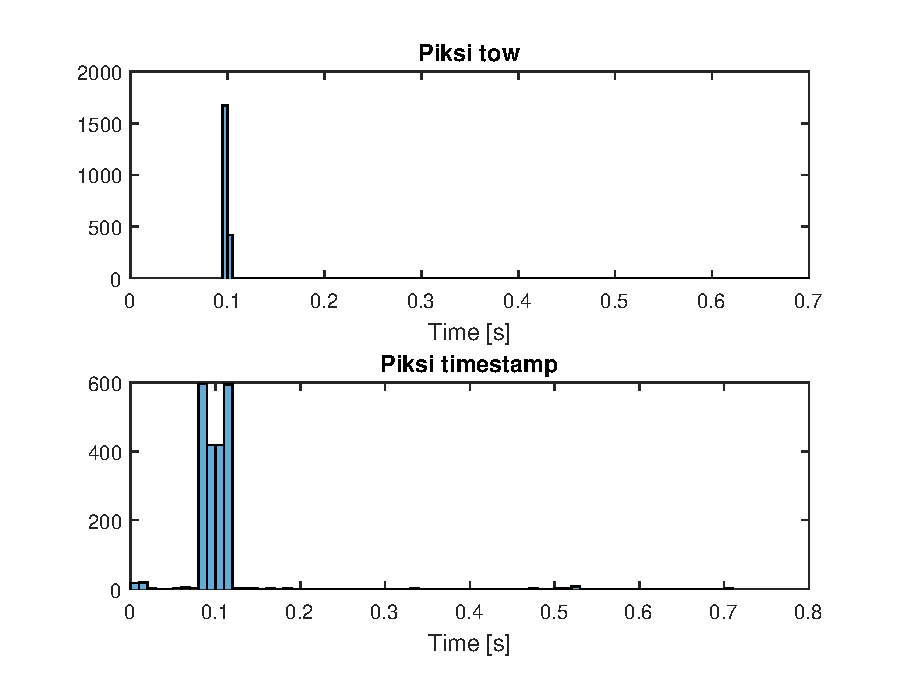
\includegraphics[width=0.7\textwidth]{figs/plots/piksitime.eps}
		\caption{The time between time samples from rtklib}
		\label{figure:timePiksiWalk1}
\end{figure}
The different receiver used in Rtklib and Piksi was not able to track the same satellites at all time. Figure \ref{figure:NumSatWalk1} shows that the Ublox LEA M8T receiver connected to Rtklib managed to track more satellite then the receiver used in Piksi.
Figure 
\begin{figure}[H]
	\centering
		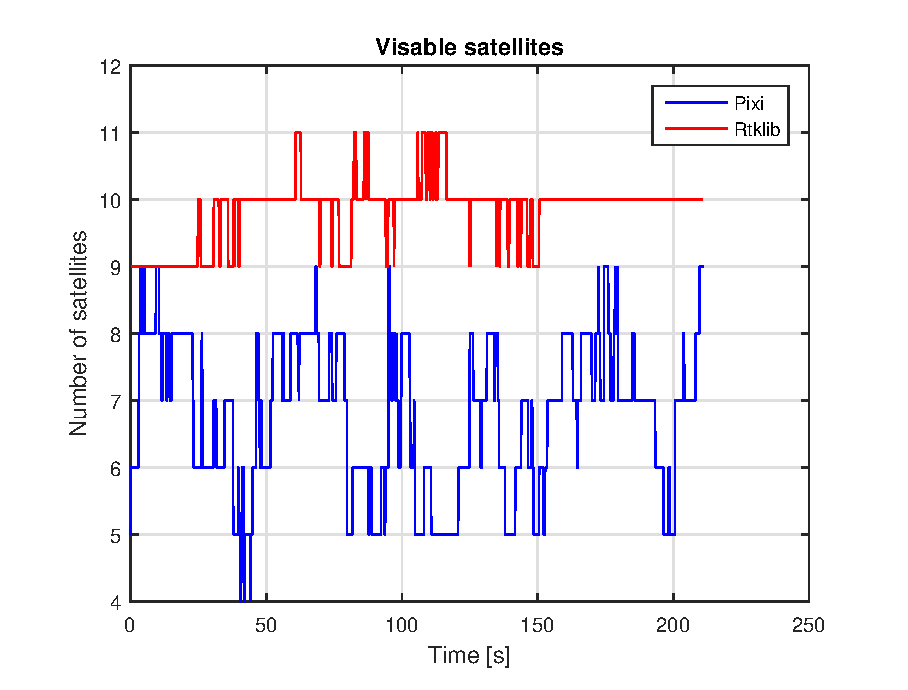
\includegraphics[width=0.7\textwidth]{figs/plots/sv.eps}
		\caption{Visable statellite for the piksi and rtklib}
		\label{figure:NumSatWalk1}
\end{figure}
\subsection{Fly test}
A test was performed at Udduvoll. Unfortunaly the test was only sucessfully with rtklib and not piksi. Because of bad weather we only managed one flight. Result shows the performance of rtklib in real time and the post processed solution from rtklib.
\cleardoublepage